  \section{Kody}

\subsection{Dwójkowo-dziesiętne (BCD)}

\subsubsection{Kod 8-4-2-1 (BCD)}

Kod 8421, znany jako BCD - kod wagowy (istnieje bezpośredni związek pomiędzy wagą a pozycją cyfry).
Wagi jak w kodzie binarnym, stąd łatwość wykonywania operacji arytmetycznych, tymi
samymi metodami, co dla liczb dwójkowych. Np. liczba 127 w kodzie 8421 będzie wyglądała tak: 0001 0010 0111 

\begin{figure}[h!]
    \centering
    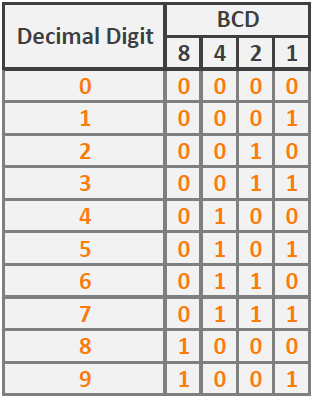
\includegraphics[width=0.35\textwidth]{images/codes/bcd.png}
    \caption{BCD}
    \label{fig:my_label}
\end{figure}

\subsubsection{Kod +3}

Kod „+3” (D = B + 3) – kod niewagowy, samouzupełniający (do 9 przez negację wszystkich bitów)

\begin{figure}[h!]
    \centering
    
\includegraphics[width=0.45\textwidth]{images/codes/plus_three.png}
    \caption{+3}
    \label{fig:my_label}
\end{figure}

\subsubsection{Kod 2-4-2-1}

Kod 2421 – kod wagowy, samouzupełniający, przydatny w układach zliczających.

\begin{figure}[h!]
    \centering
    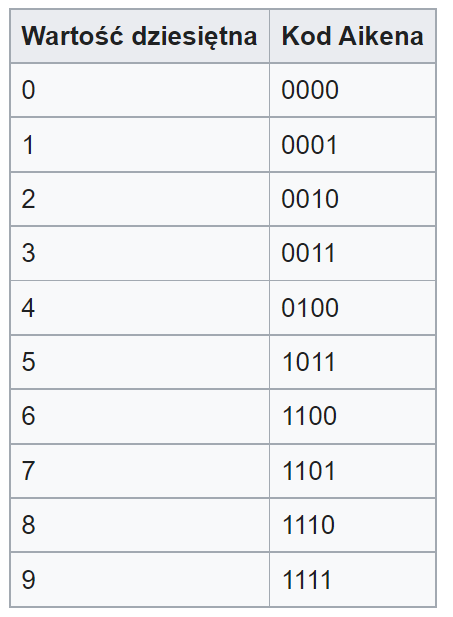
\includegraphics[width=0.4\textwidth]{images/codes/2421.png}
    \caption{2421}
    \label{fig:my_label}
\end{figure}

Wszystkie mają małą odporność na zakłócenia – np. zmiany na pozycjach mogą nie
występować jednocześnie – zmiana 0111 na 1111, zamiast na 1000 (w sterowaniu to problem).

\newpage

\subsection{Refleksyjne}

\subsubsection{Kod gray'a}

Możliwość powstawania błędów niejednoczesnej zmiany na pozycjach kodu jest
wyeliminowana w kodach, w których nie więcej niż jeden bit zmienia swoją wartość przy
przejściu między kolejnymi zakodowanymi wartościami.
Przykładem kodu refleksyjnego jest kod Graya.

\begin{figure}[h!]
    \centering
    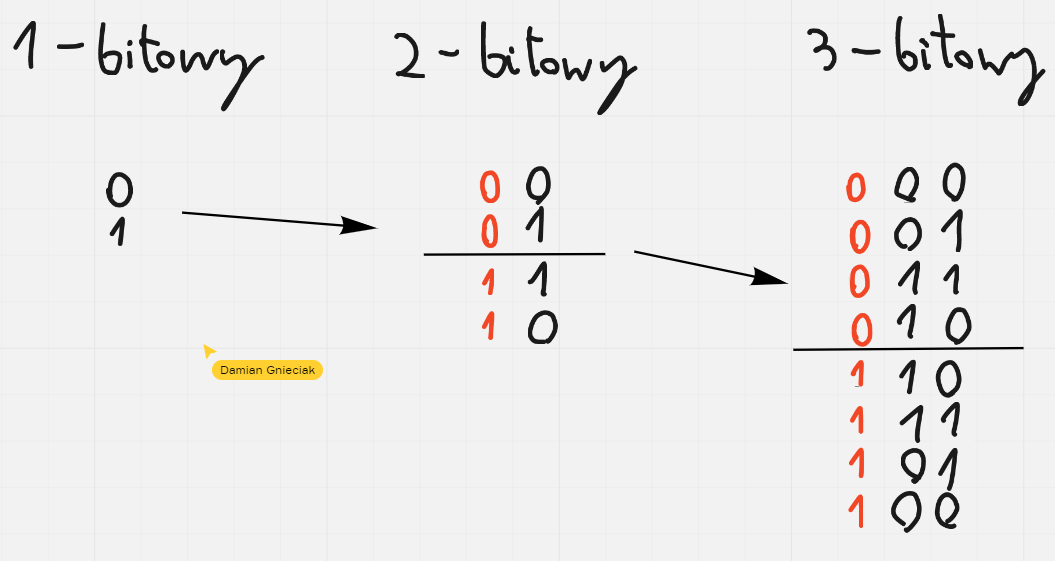
\includegraphics[width=.8\textwidth]{images/codes/kod_graya.png}
    \caption{Gray}
    \label{fig:my_label}
\end{figure}

\subsection{Detekcyjne i korekcyjne}

\subsubsection{Kod 1 z 10}

\begin{figure}[h!]
    \centering
    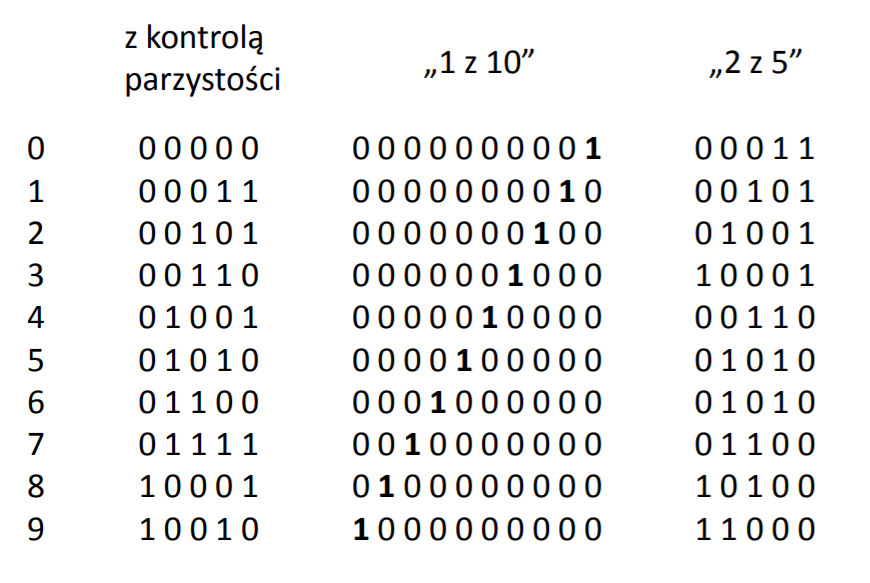
\includegraphics[width=.5\textwidth]{images/codes/detective.png}
    \caption{1 z 10}
    \label{fig:my_label}
\end{figure}

\newpage

\subsubsection{Kod 2 z 5}

\begin{figure}[h!]
    \centering
    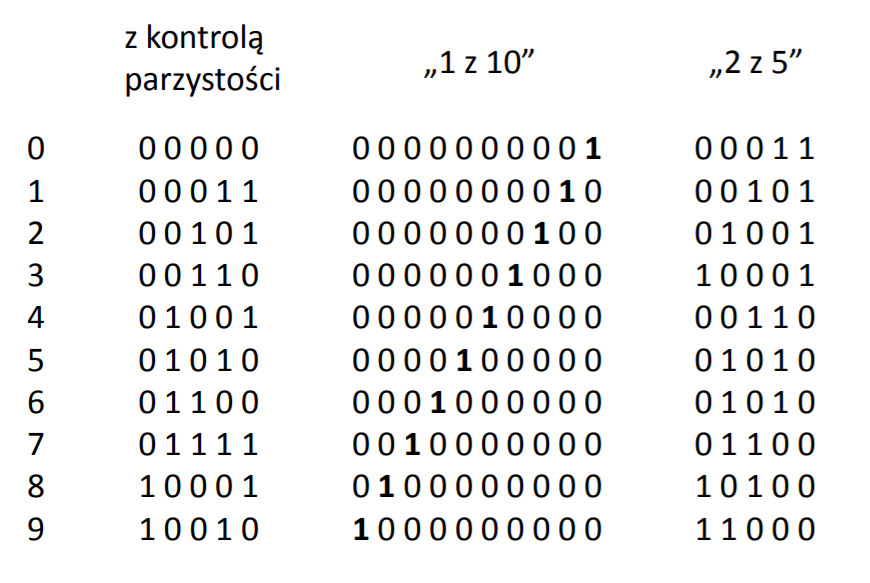
\includegraphics[width=.5\textwidth]{images/codes/detective.png}
    \caption{2 z 5}
    \label{fig:my_label}
\end{figure}

\subsubsection{Kod z kontrolą parzystości}

\begin{figure}[h!]
    \centering
    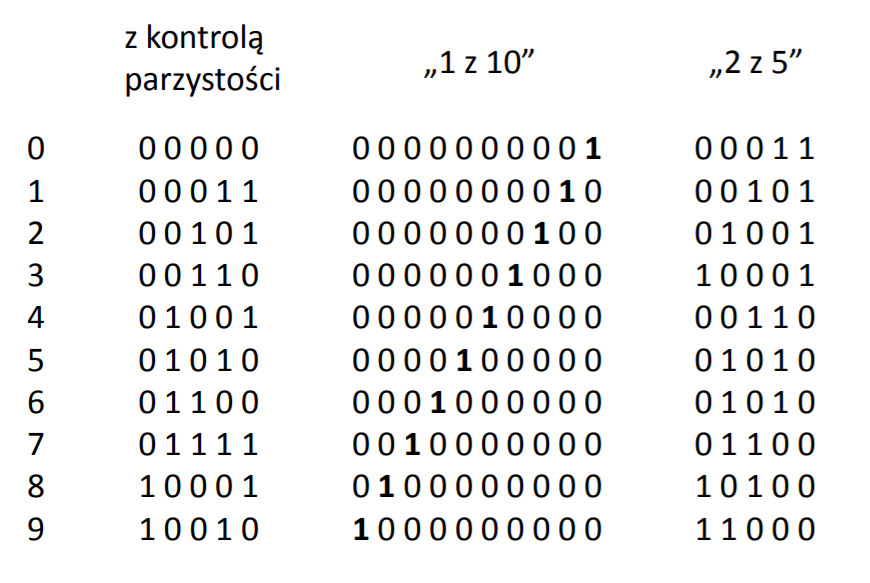
\includegraphics[width=.5\textwidth]{images/codes/detective.png}
    \caption{z kontrolą parzystości}
    \label{fig:my_label}
\end{figure}

\newpage

\subsubsection{Kod Hamming'a}

\begin{figure}[h!]
    \centering
    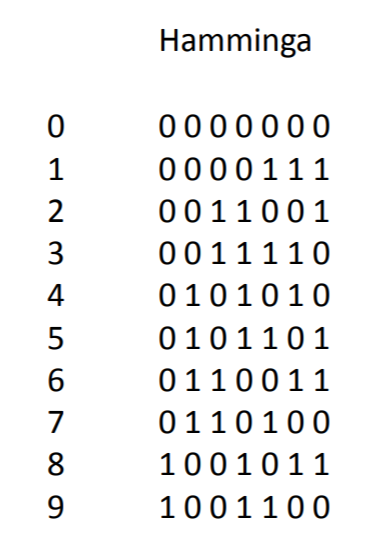
\includegraphics[width=.4\textwidth]{images/codes/hamming.png}
    \caption{Hamming}
    \label{fig:my_label}
\end{figure}